\chapter{Application: Strong Edge Colouring}
\label{chap:strong_edge_colouring}

As defined in the \hyperref[sec:intro_strong_edge_coloring]{introduction},
a strong edge colouring of a graph is an edge colouring where two edges which are incident to some
common edge must have different colours. The minimum number of colours required for a strong edge colouring of
$G$ is called the strong chromatic index $\chi'_s(G)$.
In 1985 Erd\H{o}s and Nešetřil conjectured that
$\chi'_s(G) \leq 1.25\Delta(G)^2$, and in 1989 Faudree et al. conjectured that
$\chi'_s(G) \leq \Delta(G)^2$ if $G$ is bipartite \cite{faudreeInducedMatchingsBipartite1989}.

In this chapter we will use the semidefinite method on local flags to prove the following
theorems:
\begin{knowntheorem}
    For $\Delta(G)$ large enough we have
    \[\chi'_s(G) \leq 1.73\Delta(G)^2.\]
\end{knowntheorem}
\begin{knowntheorem}
    If $G$ is bipartite then for $\Delta(G)$ large enough we have
    \[\chi'_s(G) \leq 1.6254\Delta(G)^2.\]
\end{knowntheorem}
Both of these theorems are the new improved bounds in their respective cases. We start
by showing the first result, and leave the bipartite case until section
\ref{sec:sec_bipartite}.
Additionally, in section
\ref{sec:asymmetric_bipartite_sec} we will investigate the asymmetric version of the
bipartite case, leading to an interesting discovery which suggests the strong neighbourhood
density bound coefficient is constant across all asymmetry ratios.

\section{Line Graph Equivalence}

A strong edge colouring of a graph $G$ is equivalent to a proper vertex colouring of $L(G)^2$, the
square of the line graph of $G$ (see \cite{molloyBoundStrongChromatic1997}).
The line graph $L(G)$ is a graph with a vertex $v_e$ for
each $e\in E(G)$ such that $\{v_e, v_f\} \in E(L(G))$ iff $e$ is incident to $f$ in
$G$. The square of a graph $G^2$ then is a copy of the graph where vertices at distance $\leq 2$
are connected. See figure \ref{fig:lg_example} for an example construction.

\begin{figure}[ht]
    \centering
    \includegraphics{LG_example}
    \caption{Example $G$, $L(G)$ and $L(G)^2$}
    \label{fig:lg_example}
\end{figure}

\begin{definition}[Strong Neighbourhood]
    Given a graph $G$ and edge $E \in E(G)$ define the strong neighbourhood
    $N_s(e)$ of $e$ as those edges $f \in E(G)$ which are adjacent to $e$ in 
    $L(G)^2$ (i.e. those which cannot share a colour with $e$ in a strong edge colouring).
\end{definition}

\section{The Conjecture of Erd\H{o}s and Nešetřil}

In 1985 Erd\H{o}s and Nešetřil \cite{faudreeInducedMatchingsBipartite1989} conjectured an
upper bound on the strong chromatic index $\chi'_s(G)$, the minimum colours needed for
a strong edge colouring.

\begin{conjecture}[Erd\H{o}s, Nešetřil 1985 \cite{faudreeInducedMatchingsBipartite1989}]
    $\chi'_s(G) \leq 1.25\Delta(G)^2$ for all graphs $G$.
\end{conjecture}

The bound of $2\Delta(G)^2$ was the best known bound until 1997 when Molloy and Reed
showed the following.
\begin{knowntheorem}[Molloy, Reed 1997 \cite{molloyBoundStrongChromatic1997}]
    $\chi'_s(G) \leq 1.998\Delta(G)^2$ for $\Delta(G)$ sufficiently large.
\end{knowntheorem}

Their proof consisted of colouring $L(G)^2$ with 2 discrete steps:
The first is a bound on the edge density of any neighbourhood of $L(G)^2$. We call
this the \textit{strong neighbourhood density}.
\begin{knownlemma}[Lemma 1 from \cite{molloyBoundStrongChromatic1997}]
    If $G$ has maximum degree $\Delta$ then for each $e\in E(G)$
    $|N_s(e)| \leq (1-\frac{1}{36})\binom{2\Delta^2}{2}$.
\end{knownlemma}
After showing the strong neighbourhoods in $L(G)^2$ are sparse they use a colouring
lemma to colour $L(G)^2$:
\begin{knownlemma}[Lemma 2 from \cite{molloyBoundStrongChromatic1997}]
    Let $\delta, \gamma > 0$ satisfying some condition. Then if
    $\Delta(H) \leq X$ such that $N(v)$ has at most $(1-\delta)\binom{X}{2}$ edges
    then $\chi(H)\leq (1-\gamma)X$.
\end{knownlemma}

This strategy of bounding the edge density of strong neighbourhoods of $G$ and
using a probabilistic colouring was iterated on through successive papers:
Bruhn and Joos found an asymptotically tight bound on the strong neighbourhood density
and improved the colouring lemma.
\begin{knowntheorem}[Bruhn \& Joos, 2015 \cite{bruhnStrongerBoundStrong2018}]
    $\chi'_s(G) \leq 1.93\Delta(G)^2$ for $\Delta(G)$ sufficiently large.
\end{knowntheorem}
Bonamy, Perett and Postle introduced a modification of the method where rather than
bounding the strong edge neighbourhood density for the entire graph we instead focus
on a subgraph of $L(G)^2$ of high degree vertices. They show that the
neighbourhood density in this subgraph can go below the tight bound of Bruhn and Joos
and so can be coloured with fewer colours. The rest of the graph has low degree so can
be coloured greedily.

\begin{knowntheorem}[Bonamy, Perrett \& Postle, 2018 \cite{bonamyColouringGraphsSparse2018}]
    If $\Delta(G)$ is sufficiently large then
    $\chi'_s(G) \leq 1.835\Delta(G)^2$.
\end{knowntheorem}

Most recently then Hurley, de Joannis de Verclos and Kang improved on the colouring lemma from the
Bonamy et al. paper to achieve the current lowest known bound.
\begin{knowntheorem}[Hurley, de Joannis de Verclos \& Kang, 2022 \cite{hurleyImprovedProcedureColouring2022}]
    If $\Delta(G)$ is sufficiently large then
    $\chi'_s(G) \leq 1.772\Delta(G)^2$.
\end{knowntheorem}

In this chapter we use the semidefinite method on local flags to improve the strong
neighbourhood density bound, then applying the colouring lemma from Hurley et al. as a black
box we claim the following result.

\begin{theorem}
    \label{thm:strong_edge_colouring_bound}
    If $\Delta(G)$ is sufficiently large then $\chi'_s(G) \leq 1.73\Delta(G)^2$.
\end{theorem}

The rest of this chapter is the proof of this theorem.
We will follow the same structure as used in chapter \ref{chap:pentagon_conjecture},
first reducing the problem to a problem on a certain class of coloured graphs,
finding an objective vector $O$ of local flags for which an asymptotic bound on the density of $O$ will allow
us to derive an asymptotic bound on the size of $|E(H[N_{H[F]}(f)])|$.
We then enumerate some elements
of the semantic cone and apply the semidefinite method to get a bound on $O$.

\section{Reduction}
\label{sec:sec_reduction}

The theorem that we want to improve on is the strong edge neighbourhood theorem from
the Bonamy et al. paper which appears in Hurley et al. as follows:
\begin{knowntheorem}[Theorem 3.1 \cite{hurleyImprovedProcedureColouring2022}]
    Fix $\eta \in [0, 0.3]$. For any graph $G$ let $H=L(G)^2$. Let $F$ be a
    maximal subset of $V(H)$ such that $H[F]$ has minimum degree
    $\geq (2-\eta)\Delta(G)^2$. Then for any $f\in F$ the number of edges in the subgraph
    $H[N_{H[F]}(f)]$ induced by the neighbourhood of $f$ (in $H[F]$) is at most
    \[
        \left(\frac{31}{6} - \frac{128}{10-3\eta} - \eta^2\right)\Delta(G)^4.
    \]
\end{knowntheorem}

In other words we are given a graph $G$ and a maximal subset of the edges $F \subseteq E(G)$
such that the subgraph induced by $F$ in $H=L(G)^2$ has minimum degree
$\geq (2-\eta)\Delta(G)^2$ for some $\eta$. This means each $f \in F$ has
at least $(2-\eta)\Delta(G)^2$ other edges $f' \in F$ adjacent in $L(G)^2$
($|N_s(f) \cap F| \geq (2-\eta)\Delta(G)^2\ \forall\ f \in F$).
We can then just consider the graph $H[F]$ induced by this high degree $F$ subset.
Then for some fixed $f \in F$ we want to find an upper bound on the number of edges
in its neighbourhood in $H[F]$. That is, the number of pairs $e, e' \in N_s(f) \cap F$ such
that $e, e'$ adjacent in $L(G)^2$.

\begin{note}
    The first reduction we can note is that WLOG we can assume $G$ is regular,
    as outlined in each of the above papers.
\end{note}

We note now that asymptotically it suffices to count only the number of edges
in $H[N_{H[F]}(f)]$ which correspond to pairs $e, e'\in E(G)$ which are not incident.
i.e. those $e,e'$ which are adjacent in $L(G)^2$ but not $L(G)$.
\begin{lemma}
    \label{lemma:count_non_incident_pairs}
    Let $G, F, H$ and $f\in F$ be as above. Let $A$ be those pairs $e,e'\in F$
    such that $e, e'$ adjacent in $L(G)^2$ but not $L(G)$.
    Then
    \[
        |E(H[N_{H[F]}(f)])| = |E(H[N_{H[F]}(f)]) \cap A| + o(\Delta(G)^4).
    \]
\end{lemma}
\begin{proof}
    We count how many pairs $e, e' \in N_s(f) \cap F$ are adjacent in $L(G)$.
    Clearly $|N_s(f)| \in O(\Delta(G)^2)$ and each $e \in N_s(f)$ has $O(\Delta)$
    incident edges leading to a bound of $O(\Delta(G)^3) \subseteq o(\Delta(G)^4)$
    as required.
\end{proof}

Similarly, the condition that $\deg_{H[F]}(f) \geq (2-\eta)\Delta(G)^2$ for all
$f\in F$ is dominated only by non-incident edges.
\begin{lemma}
    \label{lemma:sec_degree_non_incident}
    Let $G, F, H$ and $f\in E(G)$ be as above. Let $B$ be those edges $e\in F$
    such that $e$ is adjacent to $f$ in $L(G)^2$ but not in $L(G)$.
    Then
    \[
        \deg_{H[F]}(f) = |B| + o(\Delta(G)^2).
    \]
\end{lemma}
\begin{proof}
    The number of edges incident to a fixed $f$ in $L(G)$ is $O(\Delta(G))$.
\end{proof}

As we did in section \ref{sec:counting_pentagons} we want to reduce our problem to a
problem on coloured graphs.
Given $G$, $F\subseteq E(G)$, $\eta > 0$ and $f \in F$ as above we can construct a
new corresponding $(2,2)$-graph (red/black vertices, red/black edges) $G'$ as follows:
Let $f=\{u, v\}$. Take a copy of $G$ and colour all neighbours of $u$ and $v$ black
and all other vertices red. Then colour every edge $e \in F$ black and all other
edges red. See figure \ref{fig:transform} for example.

\begin{figure}[ht]
    \centering
    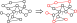
\includegraphics[scale=1]{sec_transform}
    \caption{Example coloured graph transformation}
    \label{fig:transform}
\end{figure}

\begin{lemma}
    \label{lemma:sec_black_edge_degree}
    Let $G, H=L(G)^2, F, \eta, f$ and $G'$ be as above.
    Define $E_O(G') \subseteq \binom{E(G')}{2}$ as the set of pairs of non-incident
    edges $e, e'$ in $G'$
    where $e, e'$ are black edges with a common incident edge and
    at least one of the vertices of each edge is black.
    Then the number of edges in $H[N_{H[F]}(f)]$
    where $H=L(G)^2$ is equal to $|E_O(G')| + o(\Delta(G)^4)$.
\end{lemma}

\begin{proof}
    Let $G$, $H=L(G)^2$, $F, \eta, f$ and $G'$ be as above.
    By lemma \ref{lemma:count_non_incident_pairs} it suffices to show the result for
    number of pairs $e,e'$ in $H[N_{H[F]}(f)]$ where $e,e'$ are not incident.

    Consider some edge $\{e, e'\}$ in
    $H[N_{H[F]}(f)]$ where $e,e'$ are not incident.
    Both of these $e,e'$ are in $F$ so are coloured black in $G'$.
    Similarly both are in the strong neighbourhood of $f$ meaning each has a common
    incident edge with $f$. Edges incident to $f$ have both vertices coloured black
    in $G'$ so each of $e, e'$ has at least one black vertex.
    Hence this edge $\{e, e'\}$ corresponds to a pair of non-incident black edges with at least one
    black vertex each in $G'$ at distance $\leq 2$ from each other.

    Consider then some pair $e,e' \in E_O(G')$
    As each $e,e'$ has a black vertex they must be either incident to $f$ \textit{or} equal
    to $f$. If both $e, e' \neq f$ then
    $e, e'$ satisfy exactly the conditions to be an edge in $H[N_{H[F]}(f)]$.
    Hence we overcount the number of edges in $H[N_{H[F]}(f)]$ by exactly the
    number of these pairs $e, e'\in E_0$ where one of $e, e' = f$. Assume $e=f$,
    this leaves only $\leq 2\Delta(G)^2$ choices for $e'$ so there are at most
    $2\Delta(G)^2$ such pairs which is $o(\Delta(G)^4)$ as required.
\end{proof}

\begin{corollary}
    \label{corollary:strong_density_graph_class}
    It suffices to bound the size of $E_O$
    over the class of all regular $(2,2)$-graphs where there are $\leq 2\Delta(G)^2$ black
    vertices and the subgraph of $L(G)^2$ induced by black edges has minimum
    degree $\geq (2-\eta)\Delta(G)^2$.
\end{corollary}

This is something we can bound with local flags.

\section{Local Flag Setup}

Let $\Gcl$ be the class of graphs described in corollary \ref{corollary:strong_density_graph_class}.
As before the hereditary closure $\HeredG$ only drops the regularity requirement.

\begin{lemma}
    Given the class $\Gcl$ and $\Delta$ as the max-degree function then a
    $\sigma$-flag $(F, \theta)\in \HeredG{}^\sigma$ is a local-$\sigma$ flag (definition
    \ref{def:local_flag}) iff
    each connected component of $F$ contains at least one black vertex or labelled vertex.
\end{lemma}

\begin{proof}
    See proof of lemma \ref{lemma:pentagon_local_flags}.
\end{proof}

\subsection{Objective Vector}
\label{sec:sec_obj_vector}

First we want to express the size of $E_O(G)$ as a local flag vector.
Note if $\Bcl\subseteq G$ is the set of black edges with at least one black vertex then
\[
    2|E_O(G)| = \sum_{e \in \Bcl}|\{e' \in \Bcl \colon e, e'\ \text{have common edge}\}|
\]
We can split $\Bcl$ further into $\Bcl_1$ and $\Bcl_2$, the set of edges with one
black and one red vertex and the set of edges with two black vertices respectively.
\begin{multline*}
    2|E_O(G)| = \sum_{e \in \Bcl_1}|\{e' \in \Bcl \colon e, e'\ \text{have common edge}\}|\\
    +  \sum_{e \in \Bcl_2}|\{e' \in \Bcl \colon e, e'\ \text{have common edge}\}|
\end{multline*}

The $\sigma_1=\bredge$ is a local type by lemma \ref{lemma:local_type_equiv}. Clearly
for any $e\in \Bcl_1$ we can view $G$ as a $\sigma_1$-flag where $\sigma_1$ is mapped
to $e$. Call this $G^e$. Similarly any $\sigma_1$-embedding corresponds to precisely one
$e\in \Bcl_1$.
Fix some $e\in \Bcl_1$, then take some $e'\in\Bcl$ such that $e,e'$ have a common incident edge.
Then the vertices of $e,e'$ in $G^e$ induce some subgraph of size 4 where the two unlabelled
vertices (those corresponding to $e'$) have a black edge and there is a single connected
component. Conversely any such induced subgraph corresponds to exactly one $e' \in \Bcl$.
Hence we can count such $e'$'s there are by counting how many such induced subgraphs
there are. These subgraphs are easily enumerated.

Define $D(\bredge) \in \Lcl^{\sigma_1}$ to be the vector consisting of the sum of all
local $\sigma_1$-flags of size 4 with a black edge between the unlabelled vertices and a
single connected component:
\[
    \begin{split}
        D(\bredge) &:= 
        \secdbr{5in4t2id2} + \secdbr{6in4t2id2} + \secdbr{7in4t2id2} + \secdbr{13in4t2id2} + \secdbr{14in4t2id2} + \secdbr{15in4t2id2} + \secdbr{21in4t2id2} + \secdbr{22in4t2id2} + \secdbr{23in4t2id2}\\
		& \secdbr{29in4t2id2} + \secdbr{30in4t2id2} + \secdbr{31in4t2id2} + \secdbr{37in4t2id2} + \secdbr{38in4t2id2} + \secdbr{39in4t2id2} + \secdbr{45in4t2id2} + \secdbr{46in4t2id2} + \secdbr{47in4t2id2}\\
		& \secdbr{53in4t2id2} + \secdbr{54in4t2id2} + \secdbr{55in4t2id2} + \secdbr{61in4t2id2} + \secdbr{62in4t2id2} + \secdbr{63in4t2id2} + \secdbr{74in4t2id2} + \secdbr{75in4t2id2} + \secdbr{84in4t2id2}\\
		& \secdbr{85in4t2id2} + \secdbr{86in4t2id2} + \secdbr{96in4t2id2} + \secdbr{97in4t2id2} + \secdbr{98in4t2id2} + \secdbr{108in4t2id2} + \secdbr{109in4t2id2} + \secdbr{110in4t2id2} + \secdbr{120in4t2id2}\\
		& \secdbr{121in4t2id2} + \secdbr{122in4t2id2} + \secdbr{132in4t2id2} + \secdbr{133in4t2id2} + \secdbr{134in4t2id2} + \secdbr{144in4t2id2} + \secdbr{145in4t2id2} + \secdbr{146in4t2id2} + \secdbr{156in4t2id2}\\
		& \secdbr{157in4t2id2} + \secdbr{158in4t2id2} + \secdbr{169in4t2id2} + \secdbr{170in4t2id2} + \secdbr{179in4t2id2} + \secdbr{180in4t2id2} + \secdbr{181in4t2id2} + \secdbr{191in4t2id2} + \secdbr{192in4t2id2}\\
		& \secdbr{193in4t2id2} + \secdbr{203in4t2id2} + \secdbr{204in4t2id2} + \secdbr{205in4t2id2} + \secdbr{215in4t2id2} + \secdbr{216in4t2id2} + \secdbr{217in4t2id2} + \secdbr{227in4t2id2} + \secdbr{228in4t2id2}\\
		& \secdbr{229in4t2id2} + \secdbr{239in4t2id2} + \secdbr{240in4t2id2} + \secdbr{241in4t2id2} + \secdbr{252in4t2id2} + \secdbr{253in4t2id2} + \secdbr{262in4t2id2} + \secdbr{263in4t2id2} + \secdbr{264in4t2id2}\\
		& \secdbr{274in4t2id2} + \secdbr{275in4t2id2} + \secdbr{276in4t2id2} + \secdbr{286in4t2id2} + \secdbr{287in4t2id2} + \secdbr{288in4t2id2} + \secdbr{298in4t2id2} + \secdbr{299in4t2id2} + \secdbr{300in4t2id2}\\
		& \secdbr{310in4t2id2} + \secdbr{311in4t2id2} + \secdbr{312in4t2id2} + \secdbr{323in4t2id2} + \secdbr{324in4t2id2} + \secdbr{333in4t2id2} + \secdbr{334in4t2id2} + \secdbr{335in4t2id2} + \secdbr{345in4t2id2}\\
		& \secdbr{346in4t2id2} + \secdbr{347in4t2id2} + \secdbr{357in4t2id2} + \secdbr{358in4t2id2} + \secdbr{359in4t2id2} + \secdbr{369in4t2id2} + \secdbr{370in4t2id2} + \secdbr{371in4t2id2} + \secdbr{382in4t2id2}\\
		& \secdbr{383in4t2id2} + \secdbr{392in4t2id2} + \secdbr{393in4t2id2} + \secdbr{394in4t2id2} + \secdbr{404in4t2id2} + \secdbr{405in4t2id2} + \secdbr{406in4t2id2} + \secdbr{416in4t2id2} + \secdbr{417in4t2id2}\\
		& \secdbr{418in4t2id2} + \secdbr{429in4t2id2} + \secdbr{430in4t2id2} + \secdbr{439in4t2id2} + \secdbr{440in4t2id2} + \secdbr{441in4t2id2} + \secdbr{451in4t2id2} + \secdbr{452in4t2id2} + \secdbr{453in4t2id2}\\
		& \secdbr{464in4t2id2} + \secdbr{465in4t2id2} + \secdbr{474in4t2id2} + \secdbr{475in4t2id2} + \secdbr{476in4t2id2} + \secdbr{487in4t2id2} + \secdbr{488in4t2id2}
    \end{split}
\]
Then by the above $\rho(D(\bredge); G^e) = \frac{|\{e' \in \Bcl\colon e,e'\ \text{have common edge}\}}{\binom{\Delta(G)}{2}}$.

We can then use lemma \ref{lemma:local_averaging_exp} to note that
\[
    \begin{split}
        \rho(\llbracket D(\bredge) \rrbracket; G) 
        &\sim \rho(\llbracket \bredge\rrbracket; G) \E_\theta[\rho(D(\bredge), (G,\theta))]\\
        &= \frac{1}{2}\frac{\sum_{e\in\Bcl_1}|\{e' \in \Bcl\colon e,e'\ \text{have common edge}\}|}{\binom{\Delta(G)}{2}\binom{\Delta(G)}{2}}
    \end{split}
\]

We can do the exact same construction with $\sigma_2 = \edge$. The only thing we have to note is that for any $e\in \Bcl_2$ there are two ways to embed $\sigma_2$ so defining $D(\edge)$ in
the same way we get a double count of
$\rho(D(\edge); G^e) = 2\frac{|\{e' \in \Bcl\colon e,e'\ \text{have common edge}\}}{\binom{\Delta(G)}{2}}$
hence applying lemma \ref{lemma:local_averaging_exp} again we get
\[
    \begin{split}
        \rho(\llbracket D(\edge) \rrbracket; G) 
        &\sim \rho(\llbracket \edge\rrbracket; G) \E_\theta[\rho(D(\bredge), (G,\theta))]\\
        &= \frac{\sum_{e\in\Bcl_2}|\{e' \in \Bcl\colon e,e'\ \text{have common edge}\}|}{\binom{\Delta(G)}{2}\binom{\Delta(G)}{2}}
    \end{split}
\]
Therefore
\[
    \rho(2\llbracket D(\bredge)\rrbracket + \llbracket D(\edge)\rrbracket; G)
    \sim \frac{2|E_O(G)|}{\binom{\Delta(G)}{2}\binom{\Delta(G)}{2}}
\]
so we pick $2\llbracket D(\bredge)\rrbracket + \llbracket D(\edge)\rrbracket$
as the vector we want to find a density bound for.

In general when applying the semidefinite method we will want a vector
over local flags of some fixed size $n$. Luckily our class $\Gcl$ consists of regular
graphs so we can use the extension vectors from section \ref{sec:local_flags_regular_graphs}
and corollary \ref{corollary:unlabel_extension}
to get a vector equivalent to $2\llbracket D(\bredge)\rrbracket + \llbracket D(\edge)\rrbracket$.
We define then our final objective vector $O$ to be
\[
    O := 2\left\llbracket D(\bredge) \cdot \left(\ext^\bredge_1\right)^{n-4} \right\rrbracket
        + \left\llbracket D(\edge) \cdot \left(\ext^\edge_1\right)^{n-4}\right\rrbracket
\]
for some $n\geq 4$ yet to be chosen.

\begin{lemma}
    \label{lemma:sec_objective}
    \[
        \rho(O; G) \sim \frac{2|E_O(G)|}{\binom{\Delta(G)}{2}\binom{\Delta(G)}{2}}
        \ \text{as}\ \Delta(G) \to \infty
        \ \forall\ G\in\Gcl
    \]
\end{lemma}
\begin{proof}As outlined above\end{proof}

\subsection{Search Constraints}
\label{sec:sec_search_constraints}

As in chapter \ref{chap:pentagon_conjecture}, we want to collect some known elements of
the semantic cone where each vector consists of local flags of some fixed size $n$.
(Dually this corresponds with finding linear constraints on limit functionals).
As $\Gcl$ is a class of regular graphs we get the constraints of
the form $\llbracket \ext^\sigma_i - \ext^\sigma_j\rrbracket$ from corollary
\ref{corollary:unlabel_extension} as we did in section \ref{sec:pentagon_sdp}.

First we find some constraints which encode the property
that the minimum degree of the subgraph of
$L(G)^2$ induced by black edges is $\geq (2-\eta)\Delta(G)^2$. In other words
for each black edge $e$ the number of other black edges in $G$ with a common
incident edge is $\geq (2-\eta)\Delta(G)^2$. Following how we defined $D(\bredge)$ 
we define $D'(\sigma)$ for $\sigma\in\{\edge,\bredge\}$ as the sum of
local $\sigma$-flags of size 4 where the unlabelled
vertices form a black edge. Let $e\in E(G)$ be an edge of the form $\bredge$. Then
by lemma \ref{lemma:sec_degree_non_incident} we have:
\[
    \rho(D'(\bredge); G^e) = \frac{\deg_{H[F]}(e)}{\binom{\Delta(G)}{2}} - o(1)
    \geq \frac{2\deg_{H[F]}(e)}{\Delta(G)^2} - o(1)
    \geq 2(2-\eta) - o(1)
\]
Hence $\phi(D'(\bredge)) \geq 2(2-\eta)\ \forall\ \phi \in \Phi^\bredge$.
In particular then
\[
    \begin{split}
        \phi((D'(\bredge) - 2(2-\eta)(\ext_1^\bredge)^2) \cdot \left(\ext_1^\bredge\right)^{n-4}) \geq 0
        \ \forall\ \phi \in \Phi^\bredge\\
        \implies \phi\left( \left\llbracket (D'(\bredge) - 2(2-\eta)(\ext_1^\bredge)^2) \cdot
        \left(\ext_1^\bredge\right)^{n-4}\right\rrbracket\right)\geq 0
        \ \forall\ \phi \in \Phi^\emptyset\\
    \end{split}
\]
by corollary \ref{corollary:unlabel_extension} and lemma \ref{lemma:local_pos_preserve}
giving us another constraint. We could add the same constraint for $\edge$ but in practice
it suffices to only add this one.

Next we want to encode the fact that there are at most $2\Delta(G)$ black vertices.
For any type $\sigma$ we can define the
\textit{black vertex extension vector of size $k$} $\ext_{B,k}^\sigma$ as the sum of all
local flags of size $|\sigma|+k$ where the unlabelled vertices are black vertices.

\begin{lemma}
    \label{lemma:black_extension_vector}
    For a graph $G$ let $B(G)$ denote the set of black vertices
    and $i\in \N$. Consider a $\sigma$-flag $(G, \eta)$ then
    \[
        \rho(\ext_{B,i}^\sigma; (G,\eta))
        = \frac{\binom{|B(G) \setminus \im\eta|}{i}}{\binom{\Delta(G)}{i}}
        \sim 
        \left(\frac{|B(G)\setminus\im\eta|}{\Delta(G)}\right)^i
    \]
\end{lemma}
\begin{proof}
    Consider a $\sigma$-flag $(G, \eta)$.
    Given any set of black vertices $V\subseteq B(G)\im\eta$ of size $i$ we can induce a subgraph
    $\im\eta \cup V$ of size $|\sigma|+i$ which is counted by some local $\sigma$-flag
    of size $|\sigma|+i$ where the unlabelled vertices are black. Similarly every
    $U=\im\eta \cup V$ which is isomorphic to some local $\sigma$-flag where the unlabelled
    vertices are black implies $V \subseteq B(G)\setminus\im\eta$.
\end{proof}
\begin{corollary}
    For any type $\sigma$ $\phi(\ext_{B,i}^\sigma) \leq 2^i$ for all $\phi\in\Phi^\sigma$,
    $i\in\N$.
\end{corollary}
\begin{corollary}
    For any type $\sigma$, $i\in\N$ we have $\phi(\ext_{B,i}^\sigma) = \phi(\ext_{B,1}^\sigma)^i$
\end{corollary}
\begin{corollary}
    For any type $\sigma$, $i\in [|\sigma|]$ $\phi(2\ext_i^\sigma - \ext_{B,1}^\sigma) \geq 0\ \forall
    \phi\in\Phi^\sigma$.
    If $\sigma$ is a local type then
    $\phi(\llbracket 2\ext_i^\sigma - \ext_{B,1}^\sigma\rrbracket) \geq 0\ \forall\
    \phi\in\Phi^\emptyset$.
\end{corollary}

Then we can add the constraint that
\[\llbracket 2\ext_i^\sigma - \ext_{B,1}^\sigma\rrbracket \geq 0\]
for all
local types $\sigma$ of size $n-1$. Similarly for local type $\sigma=\vertex$ we can
add the constraints
\[\phi(\llbracket (\ext_{B,1}^k - \ext_{B,k}) \cdot (\ext_1^\sigma)^{n-k-1} \rrbracket) = 0\]
for all $2 \leq k \leq n-1$ which are all constraints over flags of size $n$.

We then we add the constraint using $\sigma=\vertex$ that
$\phi(\llbracket \vertex \cdot (\ext_1^\vertex)^{n-1}\rrbracket) \leq 2$
which holds because $\llbracket \vertex \rrbracket = \vertex$.

Finally then we add the constraints of the form
$\phi(\llbracket f^2 \rrbracket) \geq 0$ for all $f\in\Lcl^\sigma$
for all local types $\sigma$. As we did in chapter \ref{chap:pentagon_conjecture} we pick a
subspace of $\Lcl^\sigma$ of flags of some size $m$ such that $f^2$ is a vector over
flags of size $n$ for each $f$ in the subspace. In particular this means $2m-|\sigma|=n$.

Letting $\Bcl=(F_1, \dots, F_\ell)$ be a list of local $\sigma$-flags of size $n$
we have the following optimisation problem:

\begin{align*}
    \max_{x\in\R^\ell}\ \ &\ \phi_x(O)\\
    \text{such that}\ \ &\ \phi_x(F_i) \geq 0\ \forall\ i \in [\ell]\\
    &\ \phi_x(\llbracket \ext^\sigma_i - \ext^\sigma_j\rrbracket) = 0\ \forall
    \ \text{local types}\ |\sigma|=n-1, i, j \in [n-1]\\
    &\ \phi_x\left( \left\llbracket (D'(\bredge) - 2(2-\eta)(\ext_1^\bredge)^2) \cdot
    \left(\ext_1^\bredge\right)^{n-4}\right\rrbracket\right)\geq 0\\
    &\ \phi_x(\llbracket 2\ext_1^\sigma - \ext_{B,1}^\sigma\rrbracket) \geq 0\ \forall
    \ \text{local types}\ |\sigma|=n-1\\
    &\ \phi_x(\llbracket (\ext_{B,1}^k - \ext_{B,k}) \cdot (\ext_1^\sigma)^{n-k-1} \rrbracket) = 0
    \ \text{for}\ \sigma=\vertex, \ \forall\ 2 \leq k \leq n-1\\
    &\ \phi_x(\llbracket f^2 \rrbracket) \geq 0 \forall f \in \Lcl_m^\sigma
    \ \forall\ \sigma\ \text{local type}\ \forall\ 2m-|\sigma|=n
\end{align*}

As with chapter \ref{chap:pentagon_conjecture} we know from section
\ref{sec:sdp_duality} how to convert this to a rigorous SDP which will find an
element $\lambda\emptyset - O \in \SemCone^\emptyset$.
This program however has a dependency on the parameter $\eta > 0$. For any fixed
value of $\eta$ we can find an upper bound on $\phi(O)$ but we cannot use this
approach to find a general closed form for such a bound in terms of $\eta$.
In practice though to prove theorem \ref{thm:strong_edge_colouring_bound}
we need only to find some ``good'' value of $\eta$. We found such an $\eta$ using
a search method described in section \ref{sec:sec_impl_notes}.

We use our SDP software (appendix \ref{app:flag_software}) and choose $n=5$ to find the following
bound:
\begin{lemma}
    \label{lemma:sec_sdp_soln}
    For $\eta = 0.2703$ we have
    \[
        10.644\emptyset - O \in \SemCone^\emptyset
    \]
\end{lemma}

We will not translate the SDP solution back to a separate proof here as we did in
section \ref{sec:pentagon_proof_validation}, instead we leave details on verifying
the construction to appendix \ref{app:sdp_verification}.

Now we can prove theorem \ref{thm:strong_edge_colouring_bound}.
\begin{proof}[Proof of theorem \ref{thm:strong_edge_colouring_bound}]
    Let $\eta = 0.2703$ and $\lambda\in\R$ be such that we have a bound of
    $\phi(O) \leq \lambda\ \forall\ \phi\in\Phi^\emptyset$.
    Then by lemma \ref{lemma:sec_objective} we have
    \[
        \lim_{\Delta(G) \to \infty}
        \frac{2|E_O(G)|}{\binom{\Delta(G)}{2}\binom{\Delta(G)}{2}}
        \leq \lambda.
    \]
    This then implies that
    \[
        \lim_{\Delta(G) \to \infty}
        \frac{|E_O(G)|}{\Delta(G)^4}
        \leq \frac{\lambda}{8}.
    \]
    We use corollary \ref{corollary:strong_density_graph_class} to translate from
    coloured graphs back to simple graphs and get that for any graph $G$,
    $H = L(G)^2$, maximal subset $F\subseteq E(G)$ such that $H[F]$ has minimum degree
    $\geq (2-\eta)\Delta(G)^2$ and some $f\in F$ we have
    \[
        \lim_{\Delta(G) \to \infty}
        \frac{|E(H[N_{H[F]}(f)])| + o(\Delta(G)^4)}{\Delta(G)^4}
        \leq \frac{\lambda}{8}
        \implies
        \lim_{\Delta(G) \to \infty}
        \frac{|E(H[N_{H[F]}(f)])|}{\Delta(G)^4}
        \leq \frac{\lambda}{8}.
    \]
    In order to apply the colouring lemma from Hurley, de Joannis de Verclos and Kang
    \cite{hurleyImprovedProcedureColouring2022} we need to find $\sigma\in\R$ such that
    $|E(H[N_{H[F]}(f)])| \leq (1-\sigma)\binom{2\Delta(G)^2}{2}$ for $\Delta(G)$ large
    enough. We can use the fact that
    $\binom{2\Delta(G)^2}{2} = 2\Delta(G)^4 - o(\Delta(G)^4)$
    to see that $\sigma = (1-\frac{\lambda}{16})$ suffices.

    Now we can apply Theorem 1.2 from Hurley et al \cite{hurleyImprovedProcedureColouring2022}
    which states that for any $\iota > 0$ there is some $\Delta_0$ large enough such that
    $\chi(H[F]) \leq (1-\varepsilon(\sigma) + \iota)2\Delta(G)^2$
    where $\varepsilon(\sigma) = \sigma/2 - \sigma^{3/2}/6$.

    Evaluating $\varepsilon(\sigma)$ for $\lambda = 10.644$ from 
    lemma \ref{lemma:sec_sdp_soln} gives a bound of
    $\chi(H[F]) \leq (1.72981 + \iota)\Delta(G)^2$
    Note then $2-\eta = 1.7297 < 1.73$ so by the proof of Theorem 1.6 in
    \cite{hurleyImprovedProcedureColouring2022}
    this proves $\chi(H) \leq 1.73\Delta(G)^2$ proving
    $\chi'_s(G) \leq 1.73\Delta(G)^2$ for $\Delta(G)$ large enough.
\end{proof}
\begin{note}
    A more careful validation of the dual solution from the SDP solver is required,
    but for the purposes of this thesis we considered it unnecessary as it is is not
    mathematically interesting. I give a brief discussion of how you can do this in
    appendix \ref{app:sdp_verification}.
    After such a validation of the floating point error you could in theory get
    a strictly below 1.73. We don't do this
    as any such result is negligibly better than 1.73 so not very interesting.
\end{note}

\subsection{Implementation Notes}
\label{sec:sec_impl_notes}

\begin{itemize}
    \item Our choice of $\eta$ here is provided above without explanation. In practice we found
        an optimal $\eta$ by a \textit{ternary search process}. Ternary search allows you to
        numerically minimise a function $f(x)$ over $x$ in some range assuming that $f$ is
        convex over that range. In particular, our choice of $\eta$ dictates our bound on
        $\chi'_s(G)$. If $\eta$ is small then $2-\eta$ is large and our bound is always $\geq
        2-\eta$. On the other hand if $\eta$ is large then we expect our strong neighbourhood
        density bound to approach the $\frac{3}{2}$ bound of Bruhn and Joos
        \cite{bruhnStrongerBoundStrong2018}. Hence we hypothesise that the bound obtained by
        choosing $\eta \in [0,2]$ is a convex function. We apply the ternary search process
        to find that $\eta=0.2703$ is a good value.
    \item The SDP program associated which finds the bound in lemma
        \ref{lemma:sec_sdp_soln} is very slow. We know by experimentation that limiting
        our class $\Gcl$ to only have red edges (those not in $F$) between black and red vertices
        gives the same bounds but is much faster. If further work is done on this problem
        with this SDP we recommend either proving we can assume this WLOG or at the very least
        ensure your derived bound is still true for the case where we don't have this limitation.
\end{itemize}

\section{The Bipartite Case}
\label{sec:sec_bipartite}

In 1989 Faudree, Gyárfas, Schelp and Tuza
made a conjecture that for the special case where $G$ is bipartite we get a tighter
upper bound on the strong chromatic index.

\begin{knownconjecture}[Faudree, Gyárfas, Schelp, Tuza \cite{faudreeInducedMatchingsBipartite1989}]
    If $G$ is bipartite then $\chi'_s(G) \leq \Delta(G)^2$.
\end{knownconjecture}

From what we can find, there are no papers showing a better bound than the general
bounds for the special case of bipartite graphs. Luckily for us the method of local flags
is easily specialised to the case of bipartite graphs meaning we can make the first
targeted progress toward this conjecture. This is a big advantage of the method of local flags,
the methods used in previous papers to bound the strong neighbourhood density do not seem
to be so easily adaptable to a special case like this.

We claim the following theorem:
\begin{theorem}
    \label{thm:sec_bipartite_bound}
    If $G$ is bipartite then for $\Delta(G)$ large enough we have
    \[\chi'_s(G) \leq 1.6254\Delta(G)^2.\]
\end{theorem}

The first thing we do is adapt our reduction from section \ref{sec:sec_reduction}. Once
again we can assume WLOG that $G$ is regular. Assume we are given
$G$, $F \subseteq E(G)$, $\eta > 0$ and $f\in F$ as before except now $G$ is bipartite.

\begin{figure}[ht]
    \centering
    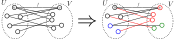
\includegraphics[scale=0.75]{bipartite_sec_transform}
    \caption{Example coloured graph transformation}
    \label{fig:bipartite_sec_transform}
\end{figure}

Once again we show how to convert $(G,F,f)$ to an equivalent coloured graph. In this case
we will use a $(4, 2)$-graph. First we pick some fixed bipartition of the vertices
of $G$, $V(G) = U \sqcup V$. This is possible as $G$ is bipartite and we can take any
such partition. Let $f=\{u,v\}$ such that $u\in U$ and $v\in V$.

Colour the neighbours of $u$ red, and the neighbours of $v$ black. Note
$N(u) \subseteq V$ and $N(v)\subseteq U$. Then colour the remaining vertices of
$U$ and $V$ blue and green respectively. Finally colour edges black if they are
$\in F$, otherwise red. See figure \ref{fig:bipartite_sec_transform} for an example.

Now, we can adopt lemmas \ref{lemma:count_non_incident_pairs} and
\ref{lemma:sec_degree_non_incident} as in the previous section.
Then we can also use the following lemma which is identical to lemma
\ref{lemma:sec_black_edge_degree}:
\begin{lemma}
    Let $G, H=L(G)^2, F, \eta, f$ and $G'$ be as above.
    Define $E_O(G') \subseteq \binom{E(G')}{2}$ as the set of pairs of non-incident
    edges $e, e'$ in $G'$
    where $e, e'$ are black edges with a common incident edge and
    at least one of the vertices of each edge is black \textbf{or red}.
    Then the number of edges in $H[N_{H[F]}(f)]$
    where $H=L(G)^2$ is equal to $|E_O(G')| + o(\Delta(G)^4)$.
\end{lemma}
\begin{proof}
    Follow the proof of lemma \ref{lemma:sec_black_edge_degree}.
\end{proof}
\begin{corollary}
    \label{corollary:bipartite_strong_density_graph_class}
    It suffices to bound the size of $E_O(G)$
    over the class $\Gcl$ of all regular $(4,2)$-graphs where there are $\Delta(G)^2$ black
    vertices, $\Delta(G)$ red vertices, the subgraph of $L(G)^2$ induced by
    black edges has minimum degree $\geq (2-\eta)\Delta(G)^2$ and the graph can be
    bi-partitioned into the components of blue/black vertices and red/green vertices.
\end{corollary}

We therefore choose our graph class $\Gcl$ as the one from
corollary \ref{corollary:bipartite_strong_density_graph_class} and as with the
previous section we get $\HeredG$ as the same class without the regularity requirement
and the following description of local flags.

\begin{lemma}
    Given the class $\Gcl$ and $\Delta$ as the maximum degree function a
    $\sigma$-flag $(F,\theta)\in\HeredG{}^\sigma$ iff each connected component
    of $F$ contains at least one black, red or labelled vertex.
\end{lemma}
\begin{proof}
    See proof of lemma \ref{lemma:pentagon_local_flags}.
\end{proof}

\subsection{Objective Vector}
\label{sec:sec_bipartite_obj}

As with section \ref{sec:sec_obj_vector} we'll define $D(\sigma)$ where
$\sigma \in \{\bredge,\blredge,\bgedge\}$ as the sum of all local $\sigma$-flags
of size 4 where the unlabelled vertices form a black edge which is connected
to the labelled vertices and at least one unlabelled vertex is red or black. Then we have:
\[
    \rho\left(\llbracket D(\bredge) \rrbracket
    + \llbracket D(\blredge) \rrbracket
    + \llbracket D(\bgedge) \rrbracket; G'\right)
    \sim \frac{|E_O(G)|}{\binom{\Delta(G)}{2}\binom{\Delta(G)}{2}}
\]
by the same derivation as in section \ref{sec:sec_obj_vector}. Hence we define
the objective vector $O$ as
\[
    O := \left\llbracket D(\bredge) \cdot \left(\ext^\bredge_1\right)^{n-4} \right\rrbracket
        + \left\llbracket D(\blredge) \cdot \left(\ext^\blredge_1\right)^{n-4}\right\rrbracket
        + \left\llbracket D(\bgedge) \cdot \left(\ext^\bgedge_1\right)^{n-4}\right\rrbracket
\]
for $n\in\N$ yet to be chosen and get the following result:
\begin{lemma}
    \label{lemma:sec_bipartite_objective}
    \[
        \rho(O; G) \sim \frac{|E_O(G)|}{\binom{\Delta(G)}{2}^2}.
    \]
    as $\Delta(G) \to \infty$ for all $G\in\Gcl$.
\end{lemma}
\begin{proof}
    As above.
\end{proof}

\subsection{Constraints}

Following the pattern of this thesis we now list some constraints on the space of
limit functionals and find ways to express them in the basis of flags of fixed size
$n$. As $\Gcl$ is a regular class we get the constraints of the form
$\phi(\llbracket \ext^\sigma_i - \ext^\sigma_j \rrbracket) = 0$ for all local types
$\sigma$, $i,j\in[|\sigma|]$. We can add these for all local $\sigma$ of size
$n-1$.

We then define $D'(\sigma)$ as we did in section
\ref{sec:sec_search_constraints} for $\sigma\in\{\bredge,\blredge,\bgedge\}$ to be
the sum of all $\sigma$-flags of size 4 where the unlabelled vertex is a black edge
connected to the labelled vertices, then again in the same construction
find that (using lemma \ref{lemma:sec_degree_non_incident})
\[\rho(D'(\sigma); G^e) \geq 2(2-\eta)-o(1)\]
for any $G\in\Gcl$, $e\in E(G)$ of type $\sigma$. Then as we did in section
\ref{sec:sec_search_constraints} we can add the following constraints to our
list:
\[
    \phi\left(\left\llbracket
    \left(D'(\sigma) - 2(2-\eta)(\ext_1^\sigma)^2\right)\cdot \left(\ext_1^\sigma\right)^{n-4}
    \right\rrbracket\right)
    \geq 0\ \forall\ \phi\in\Phi^\emptyset
\]
for all $\sigma$ above.

Finally then we add some constraints to add the fact that there are
$\Delta(G)$ black and red vertices. As we did in section
\ref{sec:sec_search_constraints} we define the
\textit{black and red vertex extension vectors of size $k$} denoted
$\ext_{B,k}^\sigma$ and $\ext_{R,k}^\sigma$ respectively, as the sum of all
local flags of size $|\sigma|+k$ where the unlabelled vertices are black
and red respectively.
Then as with lemma \ref{lemma:black_extension_vector} we get the following result:

\begin{lemma}
    For a graph $G\in\Gcl$ let $B(G)$ and $R(G)$ denote the set of black vertices and
    $k\in \N$. Then for a $\sigma$-flag $(G,\eta) \in \Gcl^\sigma$ we have
    \[
        \begin{split}
            \rho\left(\ext_{B,i}^\sigma; (G,\eta)\right)
            &= \frac{\binom{|B(G) \setminus \im\eta|}{i}}{\binom{\Delta(G)}{i}}
            \sim 
            \left(\frac{|B(G)\setminus\im\eta|}{\Delta(G)}\right)^i\\
            \rho\left(\ext_{R,i}^\sigma; (G,\eta)\right)
            &= \frac{\binom{|R(G) \setminus \im\eta|}{i}}{\binom{\Delta(G)}{i}}
            \sim 
            \left(\frac{|R(G)\setminus\im\eta|}{\Delta(G)}\right)^i.
        \end{split}
    \]
\end{lemma}
\begin{proof}
    Same as \ref{lemma:black_extension_vector}.
\end{proof}
Then as we always have $\Delta(G)$ black and red vertices we get the following:
\begin{corollary}
    For any type $\sigma$, $k\in\N$ we have $\phi(\ext_{B,k})=\phi(\ext_{R,k})=1$
    for all $\phi\in\Phi^\sigma$.
\end{corollary}
\begin{corollary}
    For any type $\sigma$, $i\in[|\sigma|]$, $k\in\N$ we have
    $\phi(\ext_1^\sigma - \ext_{B,k}) = \phi(\ext_1^\sigma - \ext_{R,k}) = 0$.
    Therefore for any local type $\sigma$
    $\phi(\llbracket \ext_1^\sigma - \ext_{B,k}\rrbracket) = \phi(\llbracket \ext_1^\sigma - \ext_{R,k}\rrbracket) = 0$.
\end{corollary}
We can add these constraints for all local types of size $n-1$.

Define $B_k, R_k$ for $k\in\N$ to be the graph of $k$ black vertices and $k$ red vertices
respectively. Then
\[
    c(B_k; G) = c(R_k; G)
    = \binom{\Delta(G)}{k}
\]
as the set of black vertices and set of red vertices are both independent.
Hence $\phi(B_k) = 1$ for all $k\in\N, \phi\in\Phi^\emptyset$. We can then do the
usual trick where we use extension vectors to project this equality
into the space of flags of size $n$.

This leaves us finally with the following optimisation problem where
$(F_1, \dots, F_\ell)$ is the ordered collection of local flags of size $n$.
\begin{align*}
    \max_{x\in\R^\ell}\ \ &\ \phi_x(O)\\
    \text{such that}\ \ &\ \phi_x(F_i) \geq 0\ \forall\ i \in [\ell]\\
    &\ \phi_x(\llbracket \ext^\sigma_i - \ext^\sigma_j\rrbracket) = 0\ \forall
    \ \text{local types}\ |\sigma|=n-1, i, j \in [n-1]\\
    &\ \phi_x\left( \left\llbracket (D'(\sigma) - 2(2-\eta)(\ext_1^\sigma)^2) \cdot
    \left(\ext_1^\sigma\right)^{n-4}\right\rrbracket\right)\geq 0\ \forall\ \sigma
    \in\{\bredge,\blredge,\bgedge\}\\
    &\ \phi_x(\llbracket \ext_1^\sigma - \ext_{B,1}^\sigma\rrbracket) = 0\ \forall
    \ \text{local types}\ |\sigma|=n-1\\
    &\ \phi_x(\llbracket \ext_1^\sigma - \ext_{R,1}^\sigma\rrbracket) = 0\ \forall
    \ \text{local types}\ |\sigma|=n-1\\
    &\ \phi_x\left(\left\llbracket B_k \cdot \left(\ext_1^{B_k}\right)^{n-k}\right\rrbracket\right)
    = 1\ \forall \ 1 \leq k \leq n\\
    &\ \phi_x\left(\left\llbracket R_k \cdot \left(\ext_1^{R_k}\right)^{n-k}\right\rrbracket\right)
    = 1\ \forall \ 1 \leq k \leq n\\
    &\ \phi_x(\llbracket f^2 \rrbracket) \geq 0 \forall f \in \Lcl_m^\sigma
    \ \forall\ \sigma\ \text{local type}\ \forall\ 2m-|\sigma|=n
\end{align*}

We then use the SDP method (appendix \ref{app:flag_software}) again to find the following
result:

\begin{lemma}
    \label{lemma:sec_bipartite_sdp_soln}
    For $\eta=0.3746$ we have
    $4.0928\emptyset - O \in \SemCone^\emptyset$
\end{lemma}

Then we can prove theorem \ref{thm:sec_bipartite_bound} exactly as we proved
theorem \ref{thm:strong_edge_colouring_bound} in the previous section.

\begin{proof}
    Let $\eta = 0.3746$ and $\lambda\in\R$ be such that we have a bound of
    $\phi(O) \leq \lambda\ \forall\ \phi\in\Phi^\emptyset$.
    Then by lemma \ref{lemma:sec_bipartite_objective} we have
    \[
        \lim_{\Delta(G) \to \infty}
        \frac{|E_O(G)|}{\binom{\Delta(G)}{2}^2}
        \leq \lambda.
    \]
    This then implies that
    \[
        \lim_{\Delta(G) \to \infty}
        \frac{|E_O(G)|}{\Delta(G)^4}
        \leq \frac{\lambda}{4}.
    \]
    We use corollary \ref{corollary:bipartite_strong_density_graph_class} to translate from
    coloured graphs back to simple graphs and get that for any bipartite graph $G$,
    $H = L(G)^2$, maximal subset $F\subseteq E(G)$ such that $H[F]$ has minimum degree
    $\geq (2-\eta)\Delta(G)^2$ and some $f\in F$ we have
    \[
        \lim_{\Delta(G) \to \infty}
        \frac{|E(H[N_{H[F]}(f)])| + o(\Delta(G)^4)}{\Delta(G)^4}
        \leq \frac{\lambda}{4}
        \implies
        \lim_{\Delta(G) \to \infty}
        \frac{|E(H[N_{H[F]}(f)])|}{\Delta(G)^4}
        \leq \frac{\lambda}{4}.
    \]
    In order to apply the colouring lemma from Hurley, de Joannis de Verclos and Kang
    \cite{hurleyImprovedProcedureColouring2022} we need to find $\sigma\in\R$ such that
    $|E(H[N_{H[F]}(f)])| \leq (1-\sigma)\binom{2\Delta(G)^2}{2}$ for $\Delta(G)$ large
    enough. We can use the fact that
    $\binom{2\Delta(G)^2}{2} = 2\Delta(G)^4 - o(\Delta(G)^4)$
    to see that $\sigma = (1-\frac{\lambda}{8})$ suffices.

    Now we can apply Theorem 1.2 from Hurley et al \cite{hurleyImprovedProcedureColouring2022}
    which states that for any $\iota > 0$ there is some $\Delta_0$ large enough such that
    $\chi(H[F]) \leq (1-\varepsilon(\sigma) + \iota)2\Delta(G)^2$
    where $\varepsilon(\sigma) = \sigma/2 - \sigma^{3/2}/6$.

    Evaluating $\varepsilon(\sigma)$ for $\lambda = 4.0928$ from 
    lemma \ref{lemma:sec_bipartite_sdp_soln} gives a bound of
    $\chi(H[F]) \leq (1.62538 + \iota)\Delta(G)^2$
    Note then $2-\eta = 1.6254$ so by the proof of Theorem 1.6 in
    \cite{hurleyImprovedProcedureColouring2022}
    this proves $\chi(H) \leq 1.6254\Delta(G)^2$ proving
    $\chi'_s(G) \leq 1.6254\Delta(G)^2$ for $\Delta(G)$ large enough.
\end{proof}

\section{Asymmetric Bipartite Strong Edge Colouring}
\label{sec:asymmetric_bipartite_sec}

In the previous section we found a bound on the strong edge colouring for bipartite
$\Delta(G)$-regular graphs. A natural question to consider is what if the graph
is bipartite, but each of the components have different maximum degrees.
Brualdi and Quinn Massey made the following conjecture
in 1993:

\begin{knownconjecture}[Brualdi, Quinn Massey \cite{brualdiIncidenceStrongEdge1993}]
    If $G=A \sqcup B$ is a bipartition then
    $\chi'_s(G) \leq \Delta(A)\Delta(B)$.
\end{knownconjecture}

In particular we will focus on the following problem: Given some
$p\in (0, 1]$ consider a bipartite graph
$G=A \sqcup B$ where $A$ is $\Delta(A)$-regular, $B$ is $\Delta(B)$-regular
and $\Delta(B) = p\Delta(A)$, what asymptotic bound can be derived on the strong chromatic
index of $G$? Clearly $p=1$ is the regular bipartite case from the previous section.

Previously, we have been using the method introduced by Bonamy, Perrett and Postle
\cite{bonamyColouringGraphsSparse2018} where we have a subset $F\subseteq E(G)$ 
with minimum degree $\geq (2-\eta)\Delta(G)^2$ in $L(G)^2$ and want to bound the
strong edge density only within this subgraph. For this section we will revert back
to the simpler method originally introduced by Molloy and Reed
\cite{molloyBoundStrongChromatic1997} where we find a general bound on the strong
neighbourhood density, then use the colouring lemma of Hurley, de Joannis de Verclos and Kang
\cite{hurleyImprovedProcedureColouring2022} to get a bound on the chromatic number.
The reason for this is that this method was more readily adapted. There is no reason
to believe that the stronger method using the high degeneracy subgraph can't be adapted
but we will see that this simpler method already reveals something very interesting about this
problem: Namely that we get the same scalar coefficient in the bound for 
$\chi'_s(G)$ for every value of $p$ we tested.

\begin{theorem}
    \label{thm:asymmetric_bipartite_bound}
    For $p\in [0.1, 0.2, 0.3, \dots, 1]$ we get the following result:
    For $\Delta(G)$ large enough where $G=A\sqcup B$ is a bipartition with
    $\Delta(B)=p\Delta(A)$ we have the bound
    \[
        \chi'_s(G) \leq 1.6632 \Delta(A)\Delta(B)
    \]
\end{theorem}

This is not a stronger result than theorem \ref{thm:sec_bipartite_bound}\footnote{This could likely
be remedied by using the method of Bonamy et. al.},
but it is extremely interesting that the different values of $p$ do not give different bounds on
$\chi'_s(G)$.

We will now give a brief description of how this was shown. We will skip the proofs as they
follow exactly as in the previous sections with minor modifications.

\subsection{Reduction}

We will follow a similar approach to section \ref{sec:sec_bipartite}. Let
$G=A \sqcup B$ be as described above and let $e=\{a, b\}\in E(G)$ be given where
$a \in A, b \in B$. We construct $G'$ a 4-coloured graph where $N(a)$ is coloured red,
$N(b)$ coloured black and the rest of $A$ and $B$ are coloured blue and green respectively
in the same fashion as figure \ref{fig:bipartite_sec_transform}. The primary thing to 
note is that we are not looking at some subgraph induced by $F\subseteq E(G)$ as before
so we do not need to introduce edge colours.

Note then $|N(a)|=\Delta(A)=\Delta(G)$ and $|N(b)|=\Delta(B)=p\Delta(G)$. Hence we
take our class $\Gcl$ to be 4-coloured bipartite graphs $G'$ which have
$\Delta(G)$ red vertices, $p\Delta(G)$ black vertices and the components of
black/blue and red/green vertices form a bipartition $G=A\sqcup B$ where
$A$, $B$ are $\Delta(G)$-regular and $p\Delta(G)$-regular respectively.

\begin{lemma}
    For any bipartite $G=A\sqcup B$ where $A$ is $\Delta(G)$ regular
    and $B$ is $p\Delta(G)$, $f\in E(G)$ we can asymptotically bound
    the strong neighbourhood density of $G$ at $f$ by any asymptotic
    bound on $|E_O(G')|$ where $G'$ is derived from $G$ by the above
    process and $E_O(G')\subseteq \binom{E(G')}{2}$
    is the set of pairs of non-incident
    edges $e,e'$ with a common incident edge and at least one vertex of both $e,e'$ 
    is red or black.
\end{lemma}

Now, these graphs $G\in\Gcl$ are no longer regular so we cannot rely on the
extension vectors from section \ref{sec:local_flags_regular_graphs} in the same way
as we have been. However, we can modify our approach slightly to take care of this issue.

For any type $\sigma$ consider vertex $i$. If $i$ is black or blue (corresponding to
component $A$) then we will still have $\phi(\ext_i^\sigma)=1$ as $A$ is
$\Delta(G)$-regular. Otherwise $i$ corresponds to a vertex in component $B$
which is $p\Delta(G)$ regular. Hence $\phi(\ext_i^\sigma)=p$. However this
implies that $\phi(\frac{1}{p}\ext_i^\sigma) = 1$. For this reason we define
the \textit{unit extension} at $i$ to be
\[
    \uext_i^\sigma = \begin{cases}
        \ext_i^\sigma & \text{if}\ i\ \text{black or blue}\\
        \frac{1}{p}\ext_i^\sigma & \text{otherwise}
    \end{cases}
\]

\begin{lemma}
    \label{lemma:asymmetric_regularity}
    For any type $\sigma$, $i,j\in [|\sigma|]$ we have
    $\phi(\uext_i^\sigma - \uext_j^\sigma) = 0$ for all
    $\phi\in\Phi^\sigma$. In particular $\llbracket \uext_i^\sigma -
    \uext_j^\sigma\rrbracket\in\SemCone^\emptyset$ if $\sigma$ is a local type.
\end{lemma}

This gives us an analogue of the $\llbracket \ext_i^\sigma - \ext_j^\sigma \rrbracket$ constraints
we have been using in our other applications.

We then follow the approach of section
\ref{sec:sec_bipartite_obj} to define $D(\sigma)$ as the sum of local
$\sigma$-flags of size 4 which are connected and at least one unlabelled vertex is
black or red. This gives us an objective vector $O$:
\begin{multline*}
O := \left\llbracket D(\bredge) \cdot \left(\uext^\bredge_1\right)^{n-4} \right\rrbracket
    + \left\llbracket D(\blredge) \cdot \left(\uext^\blredge_1\right)^{n-4}\right\rrbracket\\
    + \left\llbracket D(\bgedge) \cdot \left(\uext^\bgedge_1\right)^{n-4}\right\rrbracket
\end{multline*}
which is defined in terms of $n\in\N$ as usual.
\begin{lemma}
    For $G\in\Gcl$
    \[
        \rho(O; G) \sim \frac{|E_O(G)|}{\binom{\Delta(G)}{2}^2}
    \]
\end{lemma}

\subsection{Constraints}

First, we take the set of constraints $\phi(\llbracket \uext_i - \uext_j \rrbracket) = 0$
from lemma \ref{lemma:asymmetric_regularity}.

Next we define an \textit{black vertex extension} $\ext_B^\sigma$ and \textit{red vertex extension}
vector as in section \ref{sec:sec_search_constraints}. We then note that
as there are $\Delta(G)$ red vertices and $p\Delta(G)$ black vertices we
have $\phi(\ext_B^\sigma) = p$ and $\phi(\ext_R^\sigma)=1$ for any type
$\sigma$. We add the constraints then that
$\llbracket \ext_1^\sigma - \frac{1}{p}\ext_B^\sigma\rrbracket = 0$
and
$\llbracket \ext_1^\sigma - \ext_R^\sigma\rrbracket = 0$ for all local types
of size $n-1$.
Finally then if $B_1$, $R_1$ are the flags consisting of a single black and red
vertex we know $\phi(B_1)=p$ and $\phi(R_1)=1$ for all $\phi\in\Phi^\emptyset$.
Hence $\phi(\llbracket B_1 \cdot \uext_1^{B_1}\rrbracket) = p$ and
$\phi(\llbracket R_1 \cdot \uext_1^{R_1}\rrbracket) = 1$ are valid constraints we
can add.

\subsection{Results}
\label{sec:asymmetric_sec_results}

Using the constraints from the previous section we can construct a valid
SDP as in the other applications for some fixed $p\in (0, 1]$. Solving this
gives us a bound on the number of edges in the strong neighbourhood of the form
$|E(H[N_s(e)])| \leq \lambda_p \Delta(G)^4$.

In order to apply theorem 1.2 from Hurley et. al. \cite{hurleyImprovedProcedureColouring2022}
we need an asymptotic bound of the form $|E(H[N_s(e)])| \leq (1-\sigma)\binom{\Delta(H)}{2}$
where $H=L(G)^2$.
We can calculate that WLOG $\Delta(H)=2p\Delta(G)^2$ so $\sigma=1-\lambda_p/2p^2$
suffices. Theorem 1.2 from \cite{hurleyImprovedProcedureColouring2022} then gives
an asymptotic bound
\[
    \chi'_s(G) \leq (1-\varepsilon(\sigma)+\iota)\Delta(H)=2(1-\varepsilon(\sigma)+\iota)p\Delta(G)^2
    = 2(1-\varepsilon(\sigma)+\iota)\Delta(A)\Delta(B)
\]

Performing this process for varying values of $p$ proves
theorem \ref{thm:asymmetric_bipartite_bound}.

We found then that for every value of $p$ that we tried we would get the same
value for $\sigma$, meaning the bound on $\chi'_s(G)$ was also constant across
$p$. This suggests that the bound $\lambda_p$ is of the form $Cp^2$ for some
constant $C \approx 1.13723$.

There is a lot of interesting ways to look further into this including:
\begin{itemize}
    \item If we implement the high-degeneracy approach of Bonamy et. al. do we still get this
        constant bound across $p$?
    \item Can we generalise the SDP solution to prove that we do get the same sparsity
        bound for all $p\in (0, 1]$, rather than just experimentally trying for fixed $p$?
    \item The results of the SDP programs suggest that the supremum on the strong neighbourhood
        density is some function $\lambda_p=Cp^2$. This is a topic worth investigating in
        it's own right, to find out if this is just a limitation of the method or if there
        is some underlying truth to this assertion.
\end{itemize}
